\apendice{Especificación de Requisitos}

\section{Introducción}

En este apartado se detallan los requisitos del proyecto, destacando la importancia de establecerlos antes de iniciar la implementación. Este enfoque estructurado facilita la organización, minimiza errores y proporciona una base sólida para el desarrollo.

\section{Objetivos generales}

El proyecto tenía como objetivo abordar desafíos en el análisis de trayectorias geoespaciales mediante el desarrollo de un sistema innovador y eficiente. A continuación, se detallan los objetivos principales:

\begin{itemize}
    \item \textbf{Desarrollar un algoritmo de Big Data denominado TRA-CLUS para el análisis y agrupación de trayectorias geoespaciales.}  
    El algoritmo TRA-CLUS debía adaptarse a grandes volúmenes de datos geoespaciales, permitiendo identificar patrones y relaciones en trayectorias complejas. Este objetivo implica implementar un modelo eficiente que sea capaz de procesar datos masivos y ofrecer resultados precisos y fiables.

    \item \textbf{Facilitar la interpretación de los datos recogidos mediante representaciones gráficas claras y precisas.}  
    Con el fin de transformar datos complejos en información comprensible, se buscaba desarrollar herramientas de visualización intuitivas. Estas debían permitir a los usuarios finales analizar patrones, relaciones y tendencias de forma rápida y efectiva.

    \item \textbf{Realizar comparativas de rendimiento y precisión entre diferentes algoritmos de clustering.}  
    Este objetivo se centraba en evaluar el rendimiento del algoritmo TRA-CLUS en comparación con otros algoritmos de clustering establecidos, utilizando métricas como la eficiencia computacional, la precisión en la agrupación y la robustez frente a datos ruidosos o incompletos.

    \item \textbf{Diseñar y desarrollar una aplicación web interactiva para mostrar y analizar los resultados obtenidos por el algoritmo.}  
    La aplicación debía ofrecer una interfaz amigable que permitiera a los usuarios interactuar con los resultados del algoritmo TRA-CLUS. Además, debía incluir funcionalidades como filtros personalizados, visualización en mapas y generación de informes para facilitar el análisis y la toma de decisiones basada en datos.
\end{itemize}

Estos objetivos generales constituyen la base del proyecto, guiando el diseño y desarrollo hacia la creación de una solución integral y eficiente para el análisis de trayectorias geoespaciales.

\section{Catálogo de Requisitos}

En este apartado se desglosan los requisitos del proyecto en dos categorías principales: funcionales y no funcionales. Los requisitos funcionales describen las características que el sistema debe implementar para cumplir sus objetivos, mientras que los requisitos no funcionales detallan las restricciones y cualidades del sistema.

\subsection{Requisitos funcionales}

A continuación, se enumeran los requisitos funcionales del sistema:

\begin{itemize}

    \item \textbf{RF-1: Gestión de experimentos}
    \begin{enumerate}
        \item \textbf{RF-1.1: Navegar entre experimentos.}  
        El sistema debe permitir al usuario acceder a experimentos existentes o crear nuevos experimentos desde una página inicial.
        \item \textbf{RF-1.2: Crear y guardar experimentos.}  
        Los usuarios deben poder crear experimentos asignándoles un nombre único y guardar sus datos y resultados asociados.
        \item \textbf{RF-1.3: Almacenar datos cargados y resultados.}  
        Cada experimento debe guardar los datos cargados y los resultados generados por el algoritmo TRA-CLUS.
    \end{enumerate}

    \item \textbf{RF-2: Interacción con datos}
    \begin{enumerate}
        \item \textbf{RF-2.1: Selección de datos de entrada.}  
        El sistema debe proporcionar una página para seleccionar los clústeres que se van a usar y configurar cómo se procesarán los datos.
        \item \textbf{RF-2.2: Carga de datos.}  
        Los usuarios deben poder cargar conjuntos de datos en la aplicación para procesarlos mediante el algoritmo TRA-CLUS.
        \item \textbf{RF-2.3: Visualización de datos sin tratar.}  
        Los datos originales deben visualizarse en una página que muestre un mapa interactivo de las trayectorias cargadas.
        \item \textbf{RF-2.4: Visualización de resultados del algoritmo.}  
        Los resultados generados por el algoritmo deben representarse gráficamente en un mapa interactivo que muestre los clústeres resultantes.
        \item \textbf{RF-2.5: Análisis tabular.}  
        Los resultados deben incluirse en tablas detalladas que permitan a los usuarios analizar los datos agrupados y realizar comparaciones.
    \end{enumerate}
    
    \item \textbf{RF-3: Descarga de datos}
    \begin{enumerate}
        \item \textbf{RF-3.1: Exportar resultados.}  
        El sistema debe incluir un botón en la barra de navegación que permita descargar los resultados generados en formatos .zip.
    \end{enumerate}
    
    \item \textbf{RF-4: Borrado de un experimento existente} 
    \begin{enumerate}
        \item \textbf{RF-4.1: Eliminar un experimento previamente guardado de manera irreversible} 
        El sistema permitirá al usuario eliminar un experimento que haya sido previamente guardado en el sistema. Esta acción será irreversible, y no se podrá recuperar el experimento una vez eliminado.
        \item \textbf{RF-4.2: Asegurarse de que la eliminación es deseada por el usuario} 
		Antes de proceder con la eliminación, el sistema solicitará al usuario una confirmación adicional para evitar la eliminación accidental. Esto puede implicar un cuadro de diálogo de confirmación con opciones como "Sí, eliminar" o "Cancelar".
    \end{enumerate}

\end{itemize}

\subsection{Requisitos no funcionales}

A continuación, se detallan los requisitos no funcionales del sistema:

\begin{itemize}

    \item \textbf{RNF-1: Rendimiento}
    \begin{enumerate}
        \item \textbf{RNF-1.1: Procesamiento eficiente.}  
        La carga y el procesamiento de datos debe reducirse todo lo que sea posible para mejorar la viabilidad del algoritmo.
        \item \textbf{RNF-1.2: Renderización de mapas.}  
        Los mapas interactivos deben renderizarse sin interrupciones.
    \end{enumerate}
        \item \textbf{RNF-1.3: Optimización del algoritmo TRA-CLUS.}  
        El sistema debe avanzar en la implementación real del algoritmo TRA-CLUS, mejorando su rendimiento y asegurando su capacidad para manejar grandes volúmenes de datos geoespaciales. Este avance debe incluir optimizaciones en la precisión de los clústeres generados y en la eficiencia de procesamiento.

    \item \textbf{RNF-2: Usabilidad}
    \begin{enumerate}
        \item \textbf{RNF-2.1: Navegación intuitiva.}  
        La aplicación debe ofrecer una interfaz fácil de usar con una navegación clara entre páginas y funcionalidades.
        \item \textbf{RNF-2.2: Diseño responsivo.}  
        El sistema debe adaptarse a diferentes tamaños de pantalla, asegurando una experiencia óptima en dispositivos móviles, tablets y escritorios.
        \item \textbf{RNF-2.3: Indicadores visuales.}  
        La interfaz debe incluir indicadores que muestren el estado de carga, procesamiento y finalización de tareas.
    \end{enumerate}

    \item \textbf{RNF-3: Compatibilidad}
    \begin{enumerate}
        \item \textbf{RNF-3.1: Soporte para múltiples navegadores.}  
        La aplicación debe funcionar correctamente en los navegadores web más utilizados, como Chrome, Firefox, Edge y Safari.
        \item \textbf{RNF-3.2: Integración con formatos estándar.}  
        Los datos descargados deben ser compatibles con programas comunes como Excel y herramientas de análisis como Python o R.
    \end{enumerate}

    \item \textbf{RNF-4: Seguridad}
    \begin{enumerate}
        \item \textbf{RNF-4.1: Protección de datos.}  
        El sistema debe garantizar que los datos cargados por el usuario se mantengan seguros y no sean accesibles por terceros.
        \item \textbf{RNF-4.2: Control de errores.}  
        El sistema debe manejar errores comunes como formatos de datos incorrectos, alertando al usuario y ofreciendo posibles soluciones.
    \end{enumerate}
\end{itemize}

\section{Especificación de requisitos}

\begin{figure}[htbp]
    \centering
    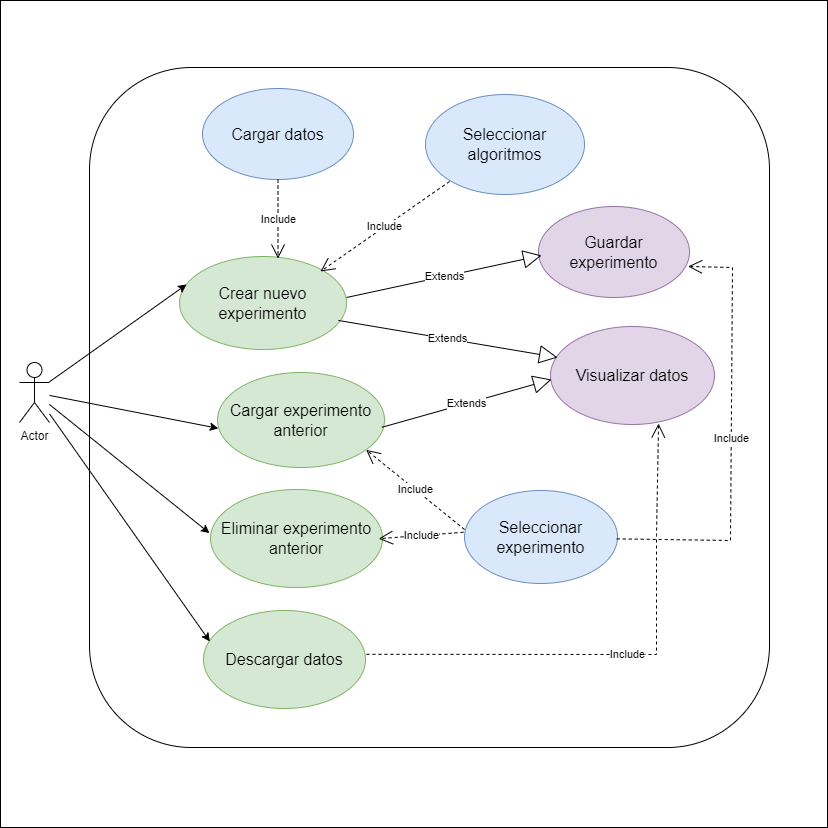
\includegraphics[width=1\linewidth]{img/Diagrama_CDU.png}
    \caption{Diagrama de casos de uso.}
    \label{Diagrama de casos de uso}
\end{figure}

En la ejecución del programa, el actor tiene tres acciones posibles: crear, cargar y descargar un experimento.

La creación de un nuevo experimento requiere que el usuario seleccione los algoritmos y los datos que se van a utilizar, lo cual incluye el paso de cargar los datos. Una vez realizados estos pasos, el nuevo experimento se guarda automáticamente y el usuario es llevado al apartado de visualización de datos.

Para cargar un experimento anterior, debe existir un experimento guardado previamente; en caso contrario, la selección del experimento (necesaria para este proceso) no será posible. Tras cargar el experimento, al igual que en la creación de uno nuevo, el usuario es dirigido al apartado de visualización de datos.

Finalmente, la descarga de un experimento solo será posible si el usuario se encuentra en el apartado de visualización, desde donde el programa permitirá realizar esta acción.

En conjunto, el sistema asegura un flujo coherente de acciones, permitiendo al usuario gestionar experimentos mediante la creación, carga, visualización y descarga de datos.

A continuación se mostrarán las tablas de uso:

\begin{table}[p]
	\centering
	\begin{tabularx}{\linewidth}{ p{0.21\columnwidth} p{0.71\columnwidth} }
		\toprule
		\textbf{CU-1}    & \textbf{Crear un nuevo experimento} \\
		\toprule
		\textbf{Versión}              & 1.0    \\
		\textbf{Autor}                & Álvaro González Delgado \\ 
		\textbf{Requisitos asociados} & RF-1, RF-2 \\
		\textbf{Descripción}          & El usuario crea un nuevo experimento seleccionando los algoritmos y los datos que se van a usar. Los datos se cargan automáticamente, y el experimento se guarda en el sistema. El usuario es dirigido a la página de visualización de datos. \\
		\textbf{Precondición}         & El sistema debe permitir crear un nuevo experimento, no debe haber restricciones previas. Se debe haber seleccionado como mínimo un experimento y rellenado sus datos. El usuario deba haber introducido un conjunto de datos balido. \\
		
		\textbf{Acciones}             &
		\begin{enumerate}
			\item El usuario accede a la página de creación de un experimento.
			\item Elige los algoritmos y variables a utilizar.
			\item Se acede a la pagina de carga de datos.
			\item Se da un nombre Y se introducen los datos.
			\item Se carga los datos.
			\item Se ejecuta el algoritmo TRA-ClUS con todas las variables introducidas.
			\item Se finaliza la carga del algoritmo.
			\item El sistema guarda el experimento automáticamente.
			\item El sistema redirige al usuario a la página de visualización de datos.
		\end{enumerate} \\
		\textbf{Postcondición}        & El experimento es guardado en el sistema y se presenta la página de visualización de datos. \\
		\textbf{Excepciones}          & Si los datos seleccionados no dan un resultado valido o hay un error de conexión el sistema muestra un error. \\
		\textbf{Importancia}          & Alta \\
		\bottomrule
	\end{tabularx}
	\caption{CU-1 Crear un nuevo experimento.}
\end{table}

\FloatBarrier

\begin{table}[p]
	\centering
	\begin{tabularx}{\linewidth}{ p{0.21\columnwidth} p{0.71\columnwidth} }
		\toprule
		\textbf{CU-2}    & \textbf{Cargar un experimento existente} \\
		\toprule
		\textbf{Versión}              & 1.0    \\
		\textbf{Autor}                & Álvaro González Delgado \\
		\textbf{Requisitos asociados} & RF-1, RF-2 \\
		\textbf{Descripción}          & El usuario carga un experimento previamente guardado. El sistema permite seleccionar un experimento de la lista disponible y lo carga para continuar con el análisis. \\
		\textbf{Precondición}         & Debe existir al menos un experimento previamente guardado. \\
		\textbf{Acciones}             &
		\begin{enumerate}
			\item El usuario elige el experimento de la lista de experimentos guardados.
			\item El sistema carga el experimento y presenta la página de visualización de datos.
		\end{enumerate} \\
		\textbf{Postcondición}        & El experimento cargado se muestra en la página de visualización de datos. \\
		\textbf{Excepciones}          & Si no existen experimentos guardados, el sistema nuestra el desplegable vació y no puede seleccionarse nada. \\
		\textbf{Importancia}          & Alta \\
		\bottomrule
	\end{tabularx}
	\caption{CU-2 Cargar un experimento existente.}
\end{table}

\FloatBarrier

\begin{table}[p]
	\centering
	\begin{tabularx}{\linewidth}{ p{0.21\columnwidth} p{0.71\columnwidth} }
		\toprule
		\textbf{CU-3}    & \textbf{Descargar los resultados de un experimento} \\
		\toprule
		\textbf{Versión}              & 1.0    \\
		\textbf{Autor}                & Álvaro González Delgado \\
		\textbf{Requisitos asociados} & RF-3 \\
		\textbf{Descripción}          & El usuario puede descargar los resultados generados por el algoritmo TRA-CLUS en formato .zip. \\
		\textbf{Precondición}         & El usuario debe estar en una de las páginas de visualización de datos. \\
		\textbf{Acciones}             &
		\begin{enumerate}
			\item El usuario accede a la página de visualización de datos cargando un experimento nuevo o guardado.
			\item El usuario presiona el botón de descarga.
			\item El sistema descarga los resultados en el formato .zip.
		\end{enumerate} \\
		\textbf{Postcondición}        & Los resultados se descargan correctamente al dispositivo del usuario. \\
		\textbf{Excepciones}          & Si no hay resultados disponibles para descargar, el sistema no hace nada. \\
		\textbf{Importancia}          & Media \\
		\bottomrule
	\end{tabularx}
	\caption{CU-3 Descargar los resultados de un experimento.}
\end{table}

\FloatBarrier

\begin{table}[p]
	\centering
	\begin{tabularx}{\linewidth}{ p{0.21\columnwidth} p{0.71\columnwidth} }
		\toprule
		\textbf{CU-4}    & \textbf{Borrar un experimento existente} \\
		\toprule
		\textbf{Versión}              & 1.0    \\
		\textbf{Autor}                & Alumno \\
		\textbf{Requisitos asociados} & RF-4 \\
		\textbf{Descripción}          & El usuario puede borrar un experimento previamente guardado. La eliminación es irreversible. \\
		\textbf{Precondición}         & El experimento debe existir previamente. \\
		\textbf{Acciones}             &
		\begin{enumerate}
			\item El usuario elige el experimento que desea borrar de la lista.
			\item El sistema despliega la petición de confirmación.
			\item El sistema elimina el experimento y confirma la eliminación.
		\end{enumerate} \\
		\textbf{Postcondición}        & El experimento es eliminado del sistema de forma irreversible. \\
		\textbf{Excepciones}          & Si el experimento no existe, el botón no racionara. \\
		\textbf{Importancia}          & Media \\
		\bottomrule
	\end{tabularx}
	\caption{CU-4 Borrar un experimento existente.}
\end{table}

\FloatBarrier